\documentclass[12pt,final,fleqn]{article}

% basic packages
\usepackage[margin=1in] { geometry }
\usepackage{amssymb,amsmath, bm}
\usepackage{verbatim}
\usepackage[latin1]{inputenc}
%\usepackage[OT1]{fontenc}
\usepackage{setspace}
\usepackage{enumitem}
\usepackage{url}
\usepackage[font={bf}]{caption}
\usepackage{float}
%\usepackage{pgfplots}
%\usepackage[font={bf}]{caption}
\usepackage{setspace}
\usepackage{latexsym}
%\usepackage{euscript}
\usepackage{graphicx}
\usepackage{marvosym}
\usepackage{amsmath} 
\usepackage{authblk}
\usepackage{xcolor}
%\usepackage[varg]{txfonts}  Older version of ``g'' in math.

% bibliography packages
\usepackage[natbibapa]{apacite}
\bibliographystyle{apacite}
\bibpunct{(}{)}{;}{a}{}{,}
\renewcommand{\bibname}{References}

% hyperref options
\usepackage{color}
\usepackage{hyperref}
\usepackage{xcolor}
\hypersetup{
    colorlinks,
    linkcolor={blue!50!black},
    citecolor={blue!50!black},
    urlcolor={blue!80!black}
}
\newcommand*{\Appendixautorefname}{Appendix}
\renewcommand*{\sectionautorefname}{Section}
\renewcommand*{\subsectionautorefname}{Section}
\newcommand{\aref}[1]{\hyperref[#1]{Appendix~\ref{#1}}}

% packages for tables
\usepackage{longtable}
\usepackage{booktabs, threeparttable}
\usepackage{threeparttablex}
%\usepackage{tabularx}
% dcolumn package
\usepackage{dcolumn}
\newcolumntype{.}{D{.}{.}{-1}}
\newcolumntype{d}[1]{D{.}{.}{#1}}
\captionsetup{belowskip=10pt,aboveskip=-5pt}
\usepackage{multirow}
% rotating package
\usepackage[figuresright]{rotating}
\usepackage{pdflscape}
\usepackage{subcaption}

% packages for figures
\usepackage{grffile}
\usepackage{afterpage}
\usepackage{float}
\usepackage[section]{placeins}


% theorem package
\usepackage{theorem}
\theoremstyle{plain}
\theoremheaderfont{\scshape}
\newtheorem{hyp}{Hypothesis}
\newtheorem{theorem}{Theorem}
\newtheorem{algorithm}{Algorithm}
\newtheorem{assumption}{Assumption}
\newtheorem{lemma}{Lemma}
\newtheorem{proposition}{Proposition}
\newtheorem{remark}{Remark}
\newcommand{\qed}{\hfill \ensuremath{\Box}}
\newcommand\indep{\protect\mathpalette{\protect\independenT}{\perp}}
\DeclareMathOperator{\sgn}{sgn}
\DeclareMathOperator{\tr}{tr}
\DeclareMathOperator{\argmin}{arg\min}
\DeclareMathOperator{\argmax}{arg\max}
\def\independenT#1#2{\mathrel{\rlap{$#1#2$}\mkern2mu{#1#2}}}
\providecommand{\norm}[1]{\lVert#1\rVert}
\renewcommand\r{\right}
\renewcommand\l{\left}
\newcommand\E{\mathbb{E}}
\newcommand\dist{\buildrel\rm d\over\sim}
\newcommand\iid{\stackrel{\rm i.i.d.}{\sim}}
\newcommand\ind{\stackrel{\rm indep.}{\sim}}
\newcommand\cov{{\rm Cov}}
\newcommand\var{{\rm Var}}
\newcommand\SD{{\rm SD}}
\newcommand\bone{\mathbf{1}}
\newcommand\bzero{\mathbf{0}}

% dotted lines in tables
%\usepackage{arydshln}

\usepackage{pdflscape}

% spacing between sections and subsections
\usepackage[compact]{titlesec}

% times new roman
%\usepackage{times}

% appendix settings
\usepackage[toc,page,header]{appendix}
\renewcommand{\appendixpagename}{\centering Appendices}
\usepackage{chngcntr}
\usepackage{etoolbox}
\usepackage{lipsum}


% file paths and definitions
\makeatletter
\newcommand*\ExpandableInput[1]{\@@input#1 }
\makeatother

\setlength{\mathindent}{1cm}
\allowdisplaybreaks[4]
\doublespacing
%\special{pdf: pagesize width 8.5truein height 11.0truein}

\titleformat{\subsection}
  {\itshape\large}{\thesubsection}{1em}{}

\setcounter{tocdepth}{1}

%--------------------------------------------------------------------------------------
% BEGIN DOCUMENT
%--------------------------------------------------------------------------------------

\begin{document}
\singlespace
\title{\textbf{Ballot initiatives and information processing, an experimental approach \\
(Pre-Analysis Plan)}\vspace{-1ex}\thanks{}}
% Direct democracy and special interest capture: experimental evidence from California
\author{Ang�le Delevoye\thanks{PhD Student in the Department of Political Science, Yale University. angele.delevoye@yale.edu}\vspace{-1ex}}
\author{Trevor Incerti\thanks{PhD Student in the Department of Political Science, Yale University. trevor.incerti@yale.edu}\vspace{-1ex}}
\affil{\textit{}\vspace{-2.5ex}}
\date{\today}
\maketitle

\begin{abstract}
\noindent
Despite representing one of the most common forms of direct democracy around the world, studies of voter persuasion efforts in ballot initiatives remain scarce. These direct democratic efforts have been hypothesized to improve the quality and legitimacy of policy decisions by some, and to lead to poor policy outcomes due to special interest capture and lack of technical knowledge by others. In order to test these hypotheses empirically, we propose a field experiment examining voting outcomes on citizen initiated ballot propositions following randomized treatment of proposition endorsement or opposition by special interest groups and policy experts during the 2020 California state elections. We seek to test whether citizens acting as policy makers give more credence to high quality policy research versus special interest information. In addition, we will replicate our field experiment with a survey experiment using identical subjects, treatments, and outcome measures.
\vspace{6cm}
\end{abstract}

\pagebreak

\doublespace


\section{Introduction} \label{sec:Introduction}

One of the most direct ways in which citizens can produce policy is through pure democratic channels such as citizens initiatives, popular consultation, and ballot initiatives. Ballot initiatives have been hailed as an efficient direct democracy mechanism, providing citizens with a much-needed voice in policy making and politics. Defenders of ballot initiatives claim that they provide a way for citizens to voice their opinions and produce policies with less interference from parties and special interests \citep{cronin1999direct}. Others caution against the excesses of direct democracy and claim that special interest capture also operates in this system \citep{rosenbluth2018responsible}. Doubts about voters' competency are also central to whether ballot initiatives lead to adoption of good policies \citep{achen2017democracy}. The need for technical knowledge may be larger on a ballot initiative than in a traditional partisan election, as fewer heuristic cues are available to voters.  

We seek to determine how voters use information when asked to vote directly on a supposedly non-partisan, technical policy proposal placed on a ballot initiative. Are voters able to distinguish between the different levels of information quality and bias that stem from varying sources of information? Relatedly, do ballot initiatives actually lead to less interference from parties and special interests, or are voters equally swayed by special interests cues and objective policy research? 

We propose a field experiment examining voting outcomes on a citizen initiated ballot proposition following randomized treatment of proposition endorsement or opposition by special interest groups and policy experts during the 2020 California elections. We seek to test whether citizens acting as policy makers give more credence to high quality policy research versus overtly partisan or biased information (i.e. special interests). In addition, we will replicate our field experiment with a survey experiment using identical subjects and treatments in order to test for replicability and/or illuminate additional mechanisms. 

The paper will also contribute to the growing literature on the effect of campaign outreach on vote choice. Meta-analysis by \citet{kalla2018minimal} suggests that the effect of campaign contact and advertising on voting outcomes is close to zero in general elections. However, effects do seem to appear in non-partisan ballot measure campaigns, but few experiments exist on this topic. Moreover, all existing ballot initiative experiments contacted voters through a single advocacy group with a clear policy position. We know little about whether the quality and/or source of the information provided changes the efficiency of these messages. 

%By contrast, our experimental design allows us to speak to the debate over whether direct democracy is actually more democratic than representative democracy, or if it suffers from the same elite manipulation might operate in both domains.
 
 A growing literature also suggests that survey experimental results often do not replicate in the field. For example, the zero effect of campaign contact in \citet{kalla2018minimal} does not replicate in survey experiments, and a recent meta analysis of the effects of providing voters with information about the corrupt actions of politicians shows an approximately zero effect in field experiments versus large negative effects in survey environments \citep{incerti2019corruption}. By contrast, we hypothesize that survey experiments should better approximate the context of real-world ballot initiatives as: (1) the vote choices are real ballot propositions rather than hypothetical candidates, and (2) partisan cues are less prevalent in (technical) ballot proposals. Whether our hypothesis is correct or incorrect, we will contribute to the growing understanding of the contexts and questions in which survey experiments replicate or do not replicate in the real world. Conducting a survey experiment will also allow us to get into potential mechanisms behind our primary outcome (voting decisions), as we will also ask the respondents factual questions on the policy topic on which they were asked to make a decision.


\section{Theory} \label{sec:Theory}

\subsection{Science, research and democracy}  \label{sec: democracy}

This project speaks to broader theoretical questions on the functioning of our current democracies, and in particular the potential gaps between reality and the ideals of deliberative democracies. We hope to contribute to ongoing discussions within philosophy of science, such as perceptions of research methods and consumption of scientific evidence outside of the academy.

\subsection{Ballot initiatives and direct democracy}

Direct democracy at the US state-level is extremely prevalent yet understudied. 31 of 50 states permit referendums of some kind, and 24 permit citizen initiatives \citep{leduc2003politics}. Of these 24 states, California engages in more individual exercises of direct democracy than any other. Since 1912 California has voted on 376 ballot initiatives at the statewide level, with a sharp rise over the past 20 years, with 139 propositions on the ballot since 1995 (only Oregon comes close to matching these numbers).

Some scholars view this growth of direct democracy as a positive extension of democratic values, providing citizens with a much-needed voice in policy making and politics. Defenders of ballot initiatives claim that they provide a way for citizens to voice their opinions and produce policies with less interference from parties and special interests \citep{cronin1999direct}. They allow the collective intelligence of the people in politics \citep{landemore2012many} to lead to better decisions. Empirically, participation in ballot initiatives is associated with an increased capacity to correctly answer factual questions about politics \citep{smith2002ballot}. There is also some evidence that voters are responsive to some types of information (synthesis of a Citizen Assembly held on the topic received in their voters pamphlets) \citep{carman2015effectiveness}. 

Others contend that the initiative process in the United States has been captured by special interest groups, directly undermining the increased power ballot initiatives are designed to deliver to citizens \citep{stratmann2004effectiveness, rosenbluth2018responsible}. Doubts about voters' competency are also central to whether ballot initiatives lead to adoption of good policies \citep{achen2017democracy}. The need for technical knowledge may be larger on a ballot initiative than in a traditional partisan election as fewer heuristic cues are available. 

This implies that the outcomes of direct democracy may be no more democratic than representative democracy, as the same elite manipulation can operate in both domains. This hypothesis is contested, however, with some observational empirical work showing a null or even negative effect of special interest spending on initiative outcomes \citep{gerber1999populist}. Our research design allows us to evaluate the special interest capture theory by comparing the efficacy of special interest messages to those of independent policy analysts.

Ballot initiatives have also been identified as a source of policy blunders. One of the most notorious is California's Proposition 13 of 1978, which capped annual increases of real property taxes to 2 percent per year and prohibited governments from increasing property taxes without a further referendum. Proposition 13 has been blamed for underfunding of California public schools, contributing to California's housing crisis, and perpetuating income inequality in the state \citep{wasi2005property, catterall1985proposition}. Proposition 13 was not without its critics at the time of passage, with critics contending that ``Proposition 13 raises serious questions about the feasibility of participatory democracy in a policy area which commonly has been dominated by experts'' \citep{mccaffery1978participatory}. In this context, our experimental design allows us to test whether voters are receptive to expert policy analysis of ballot referendum policies. 

In line with the partisan and special interest capture theories, as well as evidence that ballot initiatives often lead to policy blunders, our primary hypothesis is that \textit{voters will be equally swayed by information from special interest groups and policy researchers.} More formally, we expect the absolute value of special interest and policy research treatment effects to be statistically indistinguishable from one another.


\subsection{Current experimental evidence}  \label{sec: contact experiments}

A growing body of literature contends that information provision is relatively unsuccessful at changing voting outcomes. The primary conclusion of the Metaketa 1 project---which sought to determine if politicians were rewarded for positive information and punished for negative information---was that ``the overall effect of information [provision] across all studies is quite precisely estimated---and not statistically distinguishable from zero'' \citep{dunning2018metaketa}. In the US context, a meta-analysis by \citet{kalla2018minimal} suggests that the effect of campaign contact and advertising on voting outcomes is close to zero in general elections.

%\citet{incerti2019corruption} draws a similar conclusion in a meta-analysis of corruption information field experiments, finding no voter punishment of allegedly corrupt politicians across field experiments.

However, \citet{kalla2018minimal} find suggestive evidence that campaign contact produces positive effects on vote choice in ballot measure campaigns (see \autoref{fig: kb_meta}). While their meta-analysis includes 23 ballot initiative experiments, these experiments stem from 5 total projects \citep{arceneaux2005using, arceneaux2010comparing, rogers2015ballot}. All of these projects use advocacy groups to contact voters with a pro-initiative message via canvassing, phone, or mail. The existence of positive treatment effects in the ballot initiative environment begs the question of what kinds of informational campaigns are successful. Does high quality policy research persuade voters, or is special interest contact equally effective? 

%\citep{arceneaux2005using}: advocacy group, advocacy message, door to door canvassing, measured turnout and vote. Cluster design, precinct level.
%
%\citep{arceneaux2010comparing}: advocacy group, message tone (negative vs positive vs control), canvassing, measure turnout and vote. Two stage randomization approach, precinct level with clustering. 
%
%\citep{rogers2015ballot}: advocacy group, statewide mail program in Oregon, measure turnout and vote. 

\begin{figure}[h]
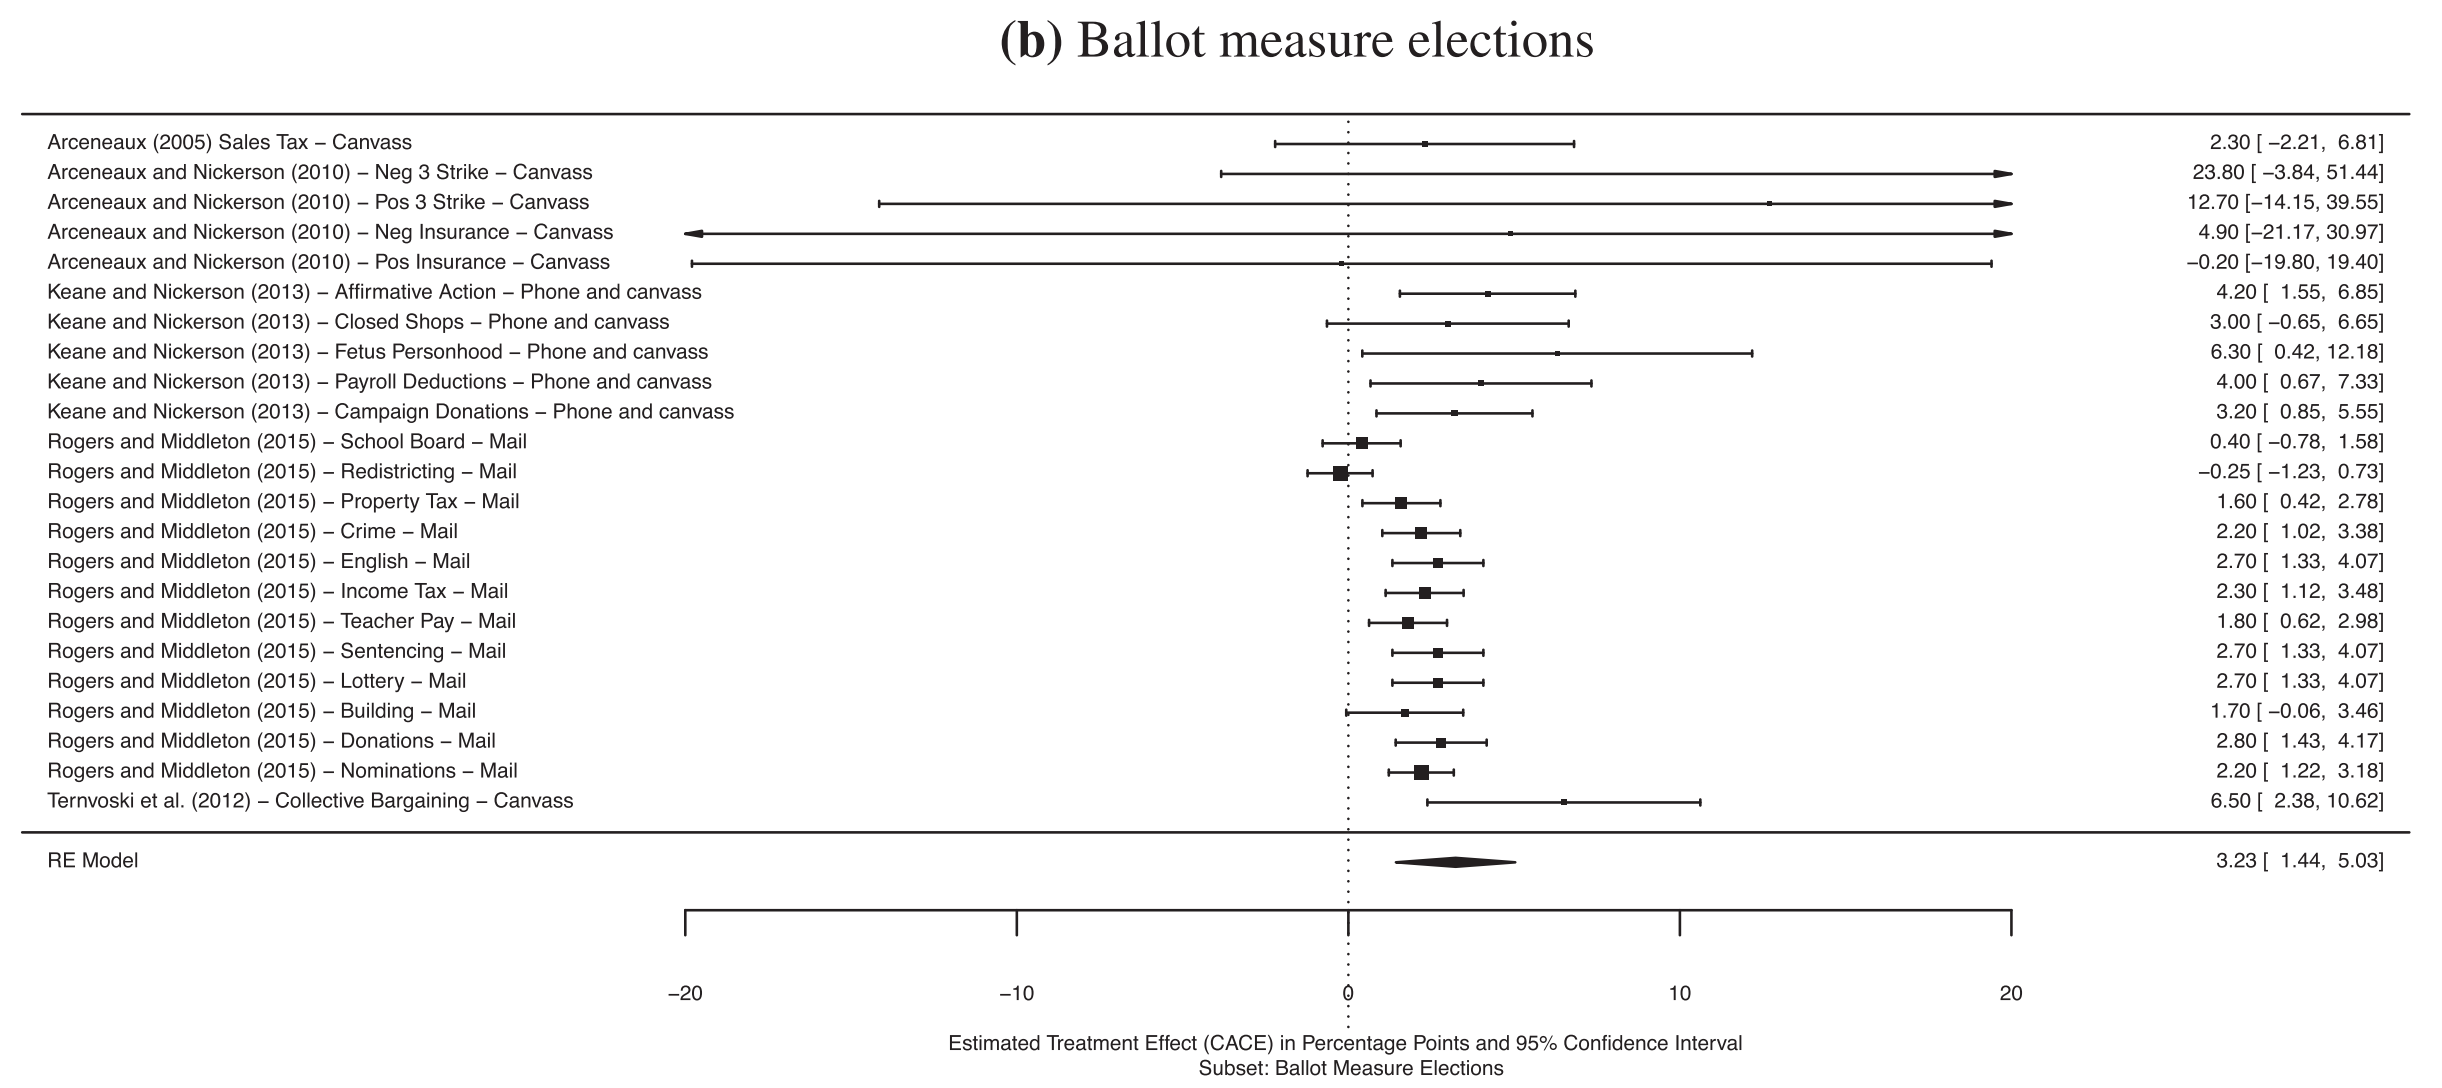
\includegraphics[scale=0.4]{meta_ballot}
\bigbreak
\caption{Meta Analysis of ballot initiative experiments from \citet{kalla2018minimal}}
\label{fig: kb_meta}
\end{figure}


\section{Field experiment} \label{sec:Design field}

\subsection{Treatment groups} \label{sec: treatment_groups}

We will provide voters with different randomized pieces of information encouraging either a ``Yes'' or ``No'' vote on a 2020 California ballot initiative. We will have three treatment groups in total: (1) placebo, (2) business/special interest group information, and (3) policy research information. Three treatment groups  allows us to have one null/zero treatment group (placebo), one positive treatment group, and one negative treatment, facilitating detection of differences between groups.

\subsection{Randomization} \label{sec: treatment_groups}

We intend to use clustered random assignment rather than individual-level randomization (i.e assigning voting precincts to treatment and control rather than individuals nested within them). \citet{arceneaux2005using} argues that clustered random assignment is simpler to implement, less expensive, and allows for direct measurement of voting outcomes without reliance on survey data.

While implementation of clustered random assignment may be simpler and allows for direct measurement of voting outcomes, analysis is more complex. If cluster size covaries with potential outcomes, the classic difference-in-means estimator will be biased. We will therefore calculate the ATE using both: (1) the classic difference-in-means estimator (while examining whether the estimated ATE changes when restricting analysis to large and small clusters), and (2) by measuring the difference in total outcomes. The latter is defined as:

$$\hat{ATE} = \frac{K_C + K_T}{N}\left(\frac{\sum Y_i(1)|d_i = 1}{K_T} - \frac{\sum Y_i(0)|d_i = 0}{K_C}\right)$$

\noindent
where $K_C$ is the number of clusters assigned to control, $K_T$ is the number of clusters assigned to treatment, $N$ is the number of subjects in the analysis, and $Y_i(1)|d_i = 1$ and $Y_i(0)|d_i = 0$ refer to potential outcomes in treatment and control clusters, respectively. Standard errors will be calculated as:

$$ \hat{SE}({\hat{ATE}}) = \sqrt{\frac{N\hat{Var}(\bar{Y}_j(0))}{K(N-m)} + \frac{N\hat{Var}(\bar{Y}_j(1))}{{Km}}} $$

\noindent
where $K$ refers to the number of clusters, $N$ refers to the total number of subjects, and $m$ refers to the total number of subjects assigned to treatment. 

Cluster-random assignment often results in a loss of statistical power. This decrease in precision increases as the difference in potential outcomes between clusters increases. To compensate, we will attempt to increase the number of clusters in our sample to the maximum extent possible while using clusters of similar size. If it becomes impossible to use clusters of similar size, we will conduct block random assignment by cluster size. We will also adjust for predictive covariates such as past voting behavior, age, gender, party registration, etc. In practice, we will therefore estimate treatment effects and standard errors using OLS regression with cluster robust standard errors and inclusive of predictive covariates, in addition to the baseline measurements described above. [Would there be anything wrong with using the most predictive covariates from the survey experiment for covariate adjustment in the field experiment?]


A potential issue with cluster random assignment at the precinct level in California is the adoption of the Voter?s Choice Act in 2016. Under the Voter's Choice Act, voters can go to any polling place in their county and can vote through mail at the county level. 5 counties opted in the system for the 2018 elections and 5 more counties are expected to do so for the 2020 elections (out of a total of 58 counties). For these counties, it means that we will not be able to get precinct-level data. We will therefore need to exclude those 10 counties (which account for 48.8\% of the California population) from our analysis. From our initial, quick look, these counties seem to be evenly distributed across partisan lines. If this methodological choice turns out to be hard to defend, we can also give up on California and conduct the experiment in another state with a significant tradition of ballot initiatives (Oregon for example). 


\subsection{Treatment details} \label{sec: treatment}

This information provision could be done through mail (a postcard), canvassing, phone calls, text messaging, or emails. Postcards, text messaging, or email would allow for larger sample sizes than canvassing or phone calls. Extant literature on fliers as a persuasive source of information finds null treatment effects \citep{kalla2018minimal, incerti2019corruption}, but the evidence in the context of ballot initiatives is more mixed. 

Moreover, it may be possible to improve upon previous field experiments by incorporating estimates of non-compliance rates into our experimental design, allowing us to estimate complier average causal effects (CACE) in addition to intent-to-treat (ITT) effects. For example, fliers could contain a link to a website with the informational treatment (ideally with some sort of monetary incentive, such as the possibility to enter a lottery). We would then be able to use the percentage of individuals who received fliers that also accessed the website as an estimate of the proportion of compliers. This would allow us to measure the effect of \textit{reading} the informational treatment, rather than the effect of being assigned to the treatment group receiving the information. 

Canvassing would provide us with less power, less geographic reach, and would likely be costlier. However, direct contact has been shown to elicit larger treatment effects than other forms of communication \citep{kalla2018minimal}.

In both cases (mail or canvassing), we will consider the possibility of partnering with a third party organization. If we send postcards for example, the source of the postcard will become a crucial part of the design. If we do not want our experiment to be about messenger effects (i.e. if we want it to be exclusively about the content, and not the source), then both treatments (interest group and expert messages) should come from the same source. We could also decide that the source of the information is part of the treatment we are interested in studying, in which case we could use different sources. 

\subsection{Outcomes} \label{sec: Outcomes}

Our outcome measurement is percentage of ``Yes'' votes on the ballot initiative at the precinct or smaller level. This constitutes a theoretically direct outcome measurement, considering that we are interested in examining how susceptible voters in a direct democracy setting are to information campaigns by different groups. 

As our outcome is ``Yes" vote and we will provide one pro-initiative treatment and one negative anti-initiative treatment, we should illicit one positive treatment effect and one negative. If the absolute values of the treatment effects are the same, or if the business treatment is higher in absolute value, that supports the capture hypothesis (i.e. people weigh both sources of information equally). If the business treatment is smaller in absolute value, it disproves the capture hypothesis and suggests that people value research more than potentially biased information.


In addition, we will look for the existence of two potential heterogeneous treatment effects: (i) partisanship of the precinct (as measured by a synthetic variable using results for federal elections over the last 10 years) and (ii) average education or income level of the precinct.


\subsection{Election cycle and choice of ballot measure} \label{sec:policy}

We seek to launch this experiment during the 2020 California statewide general election. An on-year election will give us access to a larger sample of likely voters in total, as well as a greater percentage of voters without strong priors on the specific proposal. Off-year voters tend to be more informed about specific ballot measures and therefore have stronger priors and are less susceptible to informational campaigns. 

Our ideal ballot measure would involve a policy with a scientific or policy research consensus on its overall merit or demerit. This would likely represent a technical subject on which people have relatively weak priors. Policy issues such as health care or housing could work very well for our purposes. A list of all approved 2020 state ballot initiatives can be found in \autoref{tab: state_initiatives}, and a list of approved and potential 2020 California ballot measures is provided in \autoref{tab: initiatives}.


%Treatment effect estimates will therefore be calculated as the difference-in-means of the response rate from subjects in each of treatment groups and the response rate from subjects in the control group in each block, weighted by the number of subjects in each block relative to the total number of subjects. More formally, average treatment effects will be estimated as:

%\begin{center}
%$ATE = \sum_{j = 1}^{J} \frac{N_j}{N}ATE_j$
%\end{center}

%\noindent
%where $J$ is the number of blocks, blocks are indexed by $j$, and $\frac{N_j}{N}$ represents the share of subjects who belong to block $j$. In practice, these differences-in-means will be calculated using a weighted least squares regression of response rate on treatment assignment, with weights corresponding to the inverse probability of treatment for each unit (IPW). All p-values will be calculated using randomization inference.



\subsection{Power analysis} \label{sec: power}
\citet{bloom1999using} and \citet{raudenbush1997statistical} provided excellent illustrations of power analysis for cluster random assignment. We can also rely on existing field experiments conducted during an election and using precincts as clusters. This power analysis will allow us to evaluate how many clusters (i.e. precincts) we will need to make this experiment worth conducting. 


We are still gathering data on the number of precincts and their population in California, therefore we do not present a power analysis at this stage. However, given the large number of precincts in California (more than 24.000), we do not expect power issues for this experiment.


\section{Survey experiment} \label{sec:Design survey}

\subsection{Why conduct a survey experiment?} \label{sec: questions}

Conducting a survey experiment in complement of the field experiment will provide at least two benefits: (i) to explore potential mechanisms and (ii) to contribute to the growing literature on the replicability of survey experiments results in the field. 

Substantively, a survey experiment allows us to add additional outcome variables. In addition to asking participants whether they would vote yes or no on the issue, we could ask them basic factual questions on the policy topic. If we find differences in our primary outcome (voting decision), adding this second set of outcomes could help us test whether this difference in voting can be partly explained by a difference in the understanding of the issue. \citet{knobloch2014empowering} study the impact of a Citizen Assembly in Oregon and the presence of a synthesis of the Assembly in the voters pamphlets. A state-wide survey shows that voters seemed to read and appreciate the synthesis, and they conduct a survey experiment to show that the synthesis lead to higher knowledge level on the issue than interest group or government-provided information). %But they do not study vote as the outcome variable of interest, and do not have a field experiment. 

Methodologically, a growing literature suggests that survey experimental results often do not replicate in the field. By contrast, we hypothesize that survey experiments should better approximate the context of ballot initiatives as: (1) the vote choices are real ballot propositions rather than hypothetical candidates, and (2) partisan cues are less prevalent in (technical) ballot proposals. The ballot initiative setting would allow us to design the survey so that it exactly replicates the field setting, with the only differences being hypothetical vote choice versus actual.
 
Whether our hypothesis is correct or incorrect, we will contribute to the growing understanding of the contexts and questions in which survey experiments replicate in the real world. If our hypothesis is correct, we can open the door for more survey experiments with more varied and ambitious treatments. If our hypothesis is incorrect, we show that survey experiments do not replicate even in a context where they closely approximate the field environment.

\subsection{Design} \label{sec: questions}

The ballot initiative setting would allow us to create a survey experiment in which the subjects, treatment, and outcome variable are identical to those in the field setting. In other words, we could sample from the same population, use the same informational treatments that would be sent to voters in the field setting, and measure the same outcome---vote choice---with the exception that the outcome is real in the field setting and hypothetical in the survey setting. We would then simply add a set of basic factual questions as a second set of outcomes. 

\section{Natural experiment} \label{sec:natural}

We are keeping the possibility of conduction a natural experiment on this topic open at this point, even though we have not found a specific workable design yet. The idea would be to use a real-life variation of information supply (such as data on billboards or a report sent to some precincts). The information provision will very likely not be random in this case, but we could rely on methods such as differences and differences to measure the effect of information provision on an outcome measure to be defined (vote on other measures, in previous elections, early voting, opinion polls). 

We could also potentially leverage the signature requirement thresholds to put a ballot initiative on the ballot as a discontinuity (arguing that proposals just below the threshold are substantially the same as proposals just above the threshold, and measuring the causal effect of putting a proposal to a vote through a RD design. %This would probably be another project, however, since we do not see how we can use information provision as a treatment in that case. Turnout may represent a possible outcome variable is such a discontinuity, testing if increases in the number of ballot initiatives cause more voters to go to the polls. 



\section{Conclusion} \label{sec:Conclusion}

Our next steps on this project include finalization of some of the research design decisions that remain open (i.e. choice of ballot initiative, location and creation of informational messages, possible partnership with organizations to send the messages) and the power analysis. We hope to finalize these details over the summer and to preregister a final Pre-Analysis-Plan with EGAP by the end of 2019. We would then conduct the experiment immediately prior to the 2020 California state general elections. 



\clearpage
\pagebreak
\bibliography{bibliography}

\pagebreak

\appendix
\setcounter{table}{0}
\setcounter{figure}{0}
\renewcommand\thetable{\Alph{section}.\arabic{table}}
\renewcommand\thefigure{\Alph{section}.\arabic{figure}}

\section{Appendix} \label{Appendix}


\begin{table}[!htbp] \centering 
  \caption{All currently approved 2020 ballot initiatives by state} 
  \label{tab: state_initiatives} 
\scriptsize 
\begin{tabular}{@{\extracolsep{0pt}} ccc} 
\\[-1.8ex]\hline 
\hline \\[-1.8ex] 
 & State & Title \\ 
\hline \\[-1.8ex] 
1 & Alaska & Changes to State Board of Education Amendment \\ 
2 & Alaska & Judicial System Amendment \\ 
3 & Alaska & Authorize Legislature to Recompile the State Constitution Amendment \\ 
4 & Alaska & Citizen Requirement for Voting Amendment \\ 
5 & Alaska & Judicial Vacancies Amendment \\ 
6 & Arkansas & Transportation Sales Tax Continuation Amendment \\ 
7 & Arkansas & State Legislative Term Limits Amendment \\ 
8 & Arkansas & Initiative Process and Legislative Referral Requirements Amendment \\ 
9 & California & Criminal Sentencing, Parole, and DNA Collection Initiative \\ 
10 & California & Tax on Commercial and Industrial Properties for Education and Local Government Funding Initiative \\ 
11 & California & Replace Cash Bail with Risk Assessments Referendum \\ 
12 & Colorado & Transportation Bond Issue \\ 
13 & Illinois & Allow for Graduated Income Tax Amendment \\ 
14 & Iowa & Constitional Convention Question \\ 
15 & Louisiana & No Right to Abortion in Constitution Amendment \\ 
16 & Michigan & Use of State and Local Park Funds Amendment \\ 
17 & Missouri & State Executive Term Limits Amendment \\ 
18 & Montana & LR-130, Remove Local Government Authority to Regulate Firearms Measure \\ 
19 & Montana & C-46, Initiated Amendment Distribution Requirements Measure \\ 
20 & Montana & C-47, Initiated Statute and Referendum Distribution Requirements Amendment \\ 
21 & Nebraska & Remove Slavery as Punishment for Crime Amendment \\ 
22 & Nebraska & Tax Increment Financing Repayment Amendment \\ 
23 & Nevada & Renewable Energy Standards Initiative \\ 
24 & Nevada & Marriage Regardless of Gender Amendment \\ 
25 & Nevada & State Constitutional Rights of Voters Amendment \\ 
26 & Nevada & Remove Constitutional Status of Board of Regents Amendment \\ 
27 & Nevada & State Board of Pardons Commissioners Amendment \\ 
28 & New Mexico & Appointed Public Regulation Commission Amendment \\ 
29 & North Dakota & Legislature Approval for Initiated Amendments Measure (SCR 4001) \\ 
30 & North Dakota & Amendment Changing the Membership and Terms of the Board of Higher Education (SCR 4016) \\ 
31 & Utah & Municipal Water Resources Amendment \\ 
32 & Utah & Legislator Qualifications Amendment \\ 
33 & Utah & Removal of Exception to Slavery Prohibition for Criminals Amendment \\ 
34 & Utah & Gender-Neutral Constitutional Language Amendment \\ 
35 & Wisonsin & Marsy's Law Amendment \\ 
36 & Wyoming & Constitutional Amendment A \\ 
\hline \\[-1.8ex] 
\end{tabular} 
\end{table} 


\begin{table}[!htbp] \centering 
  \caption{Potential 2020 California ballot initiatives as of June 2019}
  \label{tab: initiatives} 
  \small
\begin{tabular}{@{\extracolsep{0pt}} cccccccc} 
\\[-1.8ex]\hline 
\hline \\[-1.8ex] 
 Initiative & Topic & Endorsement & Approved & Ideal \\ 
\hline \\[-1.8ex] 
Jury trials for child custody & Legal & NA & Yes & No \\
Rental Affordability Act & Housing & NA & No & Maybe \\
Risk-based bail & Criminality & NA & No & No \\
Number of candidates in general elections & Politics & NA & No & No \\
GMO ban (SI) & Health & NA & No & Maybe \\
Fluoride ban (SI) & Health & NA & No & Maybe \\
Remove school vaccine requirement (SI) & Health & NA & No & Maybe \\
Supermajority for revenue measures & Politics & NA & No & No \\
Amend three strikes law & Criminality & NA & No & Maybe \\
Felony for some misdemeaners & Criminality & NA & No & Maybe \\
Confinement of farm animals & Agriculture & NA & No & No \\
Estate tax for college aid & Tax \& Education & NA & No & Maybe \\
No changes on approved bond spending & Politics & NA & No & Maybe \\
Elimination of Open Ended Alimony & Legal & NA & No & No \\
\hline \\[-1.8ex] 
\end{tabular} 
\end{table} 
\FloatBarrier


\end{document} 